%Hoi Perry, je toevoegingen zijn:
%-Verlet methode
%Errorberekening
%Veel errors in 2.4

\documentclass{article}
\usepackage{amsmath}
\usepackage{float}
\usepackage{amssymb}
\usepackage{graphicx}
\usepackage[margin=1in]{geometry}
\usepackage{multicol,caption,listings}
\usepackage{cite}

\bibliographystyle{plain}

\begin{document}

\title{Molecular Dynamics Simulation of Argon}
\author{P. Hansler, D. Kuitenbrouwer, and A. Lovell}
\maketitle

\noindent \textbf{Abstract}  Molecular dynamics simulations are useful in a wide variety of fields from thermodynamics to biophysics to macromolecular study.  In the 1960s, Loup Verlet performed molecular dynamics calculations on argon molecules within a Lennard-Jones potential to study their thermodynamical quantities.  In this work, we will describe the underlying structure of our own molecular dynamics simulation of argon as well as the resulting temperature, pressure, and correlation function calculations.  These will be used to investigate properties of our system and compared to previous results.  \\

\begin{multicols}{2}

\section{Introduction}

There is an increasing demand for knowledge on the dynamic properties of physical systems. Where other methods such as Monte Carlo methods are useful to find static properties of such systems, Molecular Dynamics (MD) can be used to research the dynamics of such systems. MD is based on the equations of motion. For this reason MD allows us to track down the position and momentum of each particle at each moment in time. Hence besides static properties, MD can be used to research how particles effect each other in multiple particle systems, which gives insight in the dynamics of such systems \cite{thijssen}. MD is applied in many fields, for example in biological physics in the study of macromolecules \cite{deGroot} \\

In this research, the behaviour of Argon is simulated for different values for the density and temperature. The focus of the report lies on how MD works. It is therefore discussed how to translate the physical properties of multiple particle systems, such as the Lennard-Jones potential, energy conservation, and an FCC lattice to a code. In order to get an insight in how the material behaves for different temperatures and densities, a correlation function and the pressure as function of time will be discussed. \\

This report is broken into the following sections.  In Section \ref{theory}, we will briefly discuss the theory behind the calculations in this report.  Section \ref{disc} presents the results of our calculations, including a thermostat, correlation functions for the three states of matter, and pressure calculations.  We will then give a brief conclusion in section \ref{conc}.  An appendix is found at the end of this report to discuss the method used for error analysis.  

\section{Theory}
\label{theory}

In the following sections, we will give an overview of the concepts and equations that will be needed to build a molecular dynamics simulation of argon.

\subsection{Crystalline Array}

\begin{figure}[H]
\begin{center}

\includegraphics[width=0.65\linewidth]{plots/crystal_structure.png}
\caption{Unit cell of a face-central cubic (fcc) crystal.  The entire crystal can then be built up through these unit cells.}
\label{unitcell}
\end{center}
\end{figure}

The lattice structure of argon is face-centered cubic (fcc).  The unit cell in an fcc crystal contains four atoms in the shape of a triangular pyramid, Figure \ref{unitcell}.  In the fcc lattice, the sheets of atoms stack on top of each other in such as way that every other layer is off-set by half of an atomic radius, Figure \ref{fcc}, left.  (This is in contrast to a hcp - hexagonal close packed - lattice where every other sheet of atoms lines up, Figure \ref{fcc}, right.)  \cite{crystal}  We use the fcc configuration for the initial conditions of our simulation because the equilibrium state of argon is an fcc lattice.  

\begin{figure}[H]
\begin{center}
\begin{tabular}{ c c }
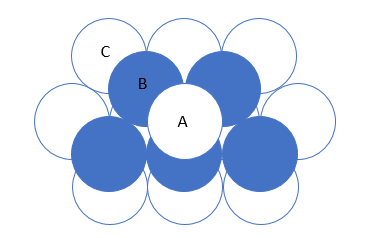
\includegraphics[width=0.45\linewidth]{plots/fcc_crystal.png} & 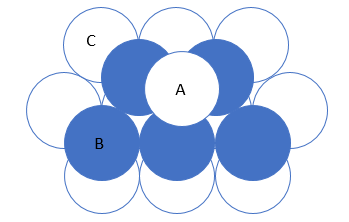
\includegraphics[width=0.45\linewidth]{plots/hcp_crystal.png}
\end{tabular}
\caption{Left, structure of an fcc crystal.  Right, structure of an hcp crystal.  In the fcc crystal, layers A and C are off-set by the radius of one of the particles in the lattice (represented by the blue and white circles).  A fourth layer on top of A would line up again with layer C.  In contrast, in the hpc structure, layers A and C directly overlap.}
\label{fcc}
\end{center}
\end{figure}

\subsection{Interaction}

To describe the interaction between each of the argon atoms, we use the Lennard-Jones potential \cite{verlet}, which accounts for the short-range repulsive force between the two atoms due to Coulomb repulsion and the longer-range attractive forces from dipole-dipole and dipole-induced dipole forces.  The form of the potential is as follows:

\begin{equation}
\label{LJpot}
V_{LJ}(r) = 4 \epsilon \left [ \left (\frac{\sigma}{r} \right )^{12} - \left (\frac{\sigma}{r} \right )^{6} \right ]
\end{equation}

\noindent where $r$ is the distance between the two atoms, $\epsilon$ gives the depth of the potential well, and $\sigma = 2R $ where $R$ is the internuclear distance between the two atoms - $\sigma$ measures the distance at which the potential between the two particles is zero.  An example of the Lennard-Jones potential can be found in Figure \ref{VLJfig}.

\begin{figure}[H]
\begin{center}
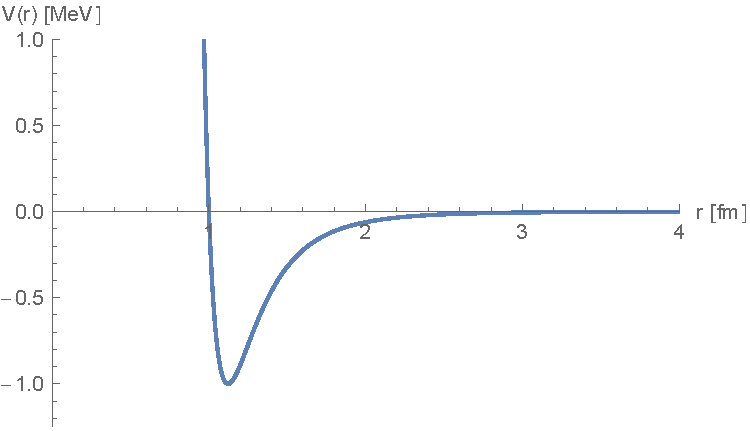
\includegraphics[width=\linewidth]{plots/VLJ.pdf}
\caption{The shape of the Lennard-Jones potential.  Here, $\sigma=1$ (where the potential crosses the r-axis) and $\epsilon =1$ (the depth of the interaction).}
\label{VLJfig}
\end{center}
\end{figure}

When the two atoms are far enough apart, they can be viewed as non-interacting.  For this reason, we can introduced a cut-off radius, $r_c$, beyond which the potential is taken to be zero.  Thus, we use the interaction 

\begin{equation}
V_{LJ} (r) = \begin{cases}
4 \epsilon \left [ \left (\frac{\sigma}{r} \right )^{12} - \left (\frac{\sigma}{r} \right )^{6} \right ] & r \le r_c \\
0 & r > r_c
\end{cases}
\end{equation}

From the expression for the Lennard-Jones potential, (\ref{LJpot}), we immediately know the form of the force between the two atoms as well.  The force is radial, acting to bring the atoms closer together if $r > r_{\mathrm{min}}$ and repelling them if $r < r_{\mathrm{min}}$, where $r_{\mathrm{min}}$ is where the potential well has its minimum (approximately 1.1 fm in Figure \ref{VLJfig}).  For our purposes, it it convenient to write the forces in terms of their Cartesian coordinates.  

\begin{equation}
\begin{split}
F_x = 24\epsilon x \left [ \frac{2 \sigma ^{12}}{r^{14}} - \frac{\sigma ^{6}}{r^8} \right ] \\
F_y = 24 \epsilon y \left [ \frac{2 \sigma ^{12}}{r^{14}} - \frac{\sigma ^{6}}{r^8} \right ] \\
F_z = 24 \epsilon z \left [ \frac{2 \sigma ^{12}}{r^{14}} - \frac{\sigma ^{6}}{r^8} \right ] \\
\end{split}
\end{equation}

\noindent From the force between each pair of particles, the momenta and positions can be calculated, leading to the dynamics of the system.  This also allows calculation of thermodynamical quantities, such as pressure and correlation functions.\\

\subsection{Velocity Verlet Method}

The method chosen for the position and momentum calculations is the Verlet method.  While both can be calculated from introductory physics equations,

\begin{equation}
\label{momeqn}
p_{i+1}=p_i + F \Delta t
\end{equation}

\noindent and

\begin{equation}
\label{poseqn}
x_{i+1} = x_i + \frac{p_i}{m} + \frac{1}{2}\frac{F(\Delta t)^2}{m}
\end{equation}

\noindent this can lead to numerical inaccuracies in the position calculation because of the dependence on the square of the time step and both the previous force and momentum. Therefore, in our algorithm we make use of the Verlet method due to its accuracy, stability and its tendency to traject the same path in phase space within numerical precision. In our simulation we will need the momenta and positions at every time step to calculate parameters such as energy. A variety of the Verlet method which accomplishes this is known as the Verlet velocity scheme \cite{verlet}.

% link: http://www.physics.udel.edu/~bnikolic/teaching/phys660/numerical_ode/node5.html

\begin{equation}
\label{verletvscheme}
\begin{split}
p_{i+\frac{1}{2}}=p_i + \frac{F_i}{2} \Delta t \\
r_{i+1}=r_i+\frac{p_{i+\frac{1}{2}}}{m} \Delta t \\
F_{i+1}=-\frac{1}{m} \frac{\partial V_{LJ}(r_i)}{\partial r} \\
p_{i+1} = p_{i+\frac{1}{2}} + \frac{F_{i+1}}{2} \Delta t \\
\end{split}
\end{equation}

\subsection{Thermodynamics}
\label{thermo}

Along with updating the position an momentum of each particle to see how the system equilibrates, there are also several thermodynamic quantities that we can calculate in order to learn more about the system we have created.  Before calculating any quantities, we want to model our system as being in contact with a thermostat to keep it at a constant temperature.  We do this by renormalizing the velocity.  \\

Through the Equipartition Theorem, the average velocity and temperature of a system are related by

\begin{equation}
\label{vir}
\frac{1}{2}m \langle v^2 \rangle = \frac{3}{2} k_B T
\end{equation}

\noindent where $m$ is the mass of the system, $\langle v^2 \rangle$ is the time average of the square of the velocity, $k_B$ is Boltzmann's constant (equal to one in a system where we take temperature and energy to have the same unit), and $T$ is the temperature of the system.  Therefore, to enforce a target temperature, $T_o$ in our system, the system must have a certain average velocity, $\langle v^2 \rangle _o$ given by

\begin{equation}
\label{virknot}
\frac{1}{2}m \langle v^2 \rangle _o = \frac{3}{2} k_B T_o
\end{equation}

Dividing (\ref{vir}) by (\ref{virknot}) and taking the square root of each side, we have

\begin{equation}
\sqrt{\frac{\langle v^2 \rangle}{\langle v^2 \rangle _o}} = \left ( \frac{T}{T_o} \right ) ^{1/2}
\end{equation}

\noindent Thus we can renormalize each velocity with 

\begin{equation}
v = \lambda v_o
\end{equation}

\noindent where $\lambda = (T/T_o)^{1/2}$ to ensure a constant temperature.  \\

To calculate the temperature of a system, we again make use of the Equipartition Theorem (\ref{vir}), taking into account the number of particles in the system in the following way

\begin{equation}
\frac{1}{2}N m \langle v^2 \rangle = \frac{3}{2} (N-1) k_B T
\end{equation}

\noindent The temperature of the system is then found by rearranging the above equation

\begin{equation}
T = \frac{Nm \langle v^2 \rangle}{3(N-1)k_B}
\end{equation}

\noindent which can easily be written in terms of the total kinetic energy of the system $E_{kin} = \frac{N}{2} \langle v^2 \rangle $.  \\

Once the system is at a constant temperature, we can calculate the correlation function.  The correlation function measures the amount of disorder in a system, and therefore gives a distinct shape based on the state of matter - solid, liuqid or gas.  To calculate the correlation function, $g(r)$, we count the number of particles inside a spherical shell of $r + \delta r$ and normalize by the volume of that shell.  Taking $\delta r$ to be much smaller than $r$, we can approximate the volume of each shell by

\begin{equation}
\begin{split}
\Delta V & = \frac{4}{3} \pi (r+\delta r)^3 - \frac{4}{3} \pi r^3 \\
& = \frac{4}{3} \pi \left [ r^3 \left (1+\frac{\delta r}{r} \right )^3 - r^3 \right ] \\
& = \frac{4}{3} \pi \left [ r^3 \left ( 1 + 3\frac{\delta r}{r} + \mathcal{O} (\delta r ^2) \right ) - r^3 \right ] \\
& = 4 \pi r^2 \delta r
\end{split}
\end{equation}

\noindent where the third line uses the Taylor approximation of $(1+z)^n = 1 + nz+ ...$  Thus the correlation function is

\begin{equation}
g(r) = \frac{N_r}{4 \pi r^2 \delta r}
\end{equation}

\noindent where $N_r$ is the number of particles found in the shell $r + \delta r$.  \\

The correlation function has distinct shapes for each state of matter.  Solids are classified by period spikes which indicates a lattice of particles.  Liquids look like a decaying periodic function.  Lastly, gases show an exponential-like decay in their correlation function.  These are the characteristics we will be looking to explore in our calculations. \\

%\noindent Another physical quantity that can be calculated is the pressure. The pressure can be calculated by making use of the following formula:

%\begin{equation}
%  = \frac{NK_{B}T}{V} + \frac{1}{3V}\avg{\sum\limits_{i}^N %R_{ij}\frac{\partial u(r)}{\partial R_{ij}}} - \frac{2$\pi%$N^2}{3V^2}\int_R_{c}^\inf\! R^3 \frac{\partial u(r)}{\partial R}g(r)dR
%\end{equation}

Another physical quantity that can be calculated is the pressure.  With a constant temperature, the pressure of a system can be found using the Virial Theorem.  Using Hamilton's equations

\begin{equation}
\begin{split}
\dot{\textbf{r}}_a = \textbf{v}_a \\
\dot{\textbf{p}}_a = \textbf{F}_a 
\end{split}
\end{equation}

\noindent and taking the time average of $\sum \limits _a (\textbf{r}_a \cdot \textbf{p}_a)$, we have

\begin{equation}
\begin{split}
\overline{\frac{d}{dt} \sum \limits _a \textbf{r}_a \cdot \textbf{p}_a} & = \overline{\sum \limits _a \textbf{v}_a \cdot \textbf{p}_a + \textbf{r}_a \cdot \textbf{F}_a} \\
& = 0
\end{split}
\end{equation}

\noindent  For non-relativistic particles 

\begin{equation}
K = \sum \limits _a \frac{\textbf{p}_{a}^2}{2m_a}
\end{equation}

\noindent and 

\begin{equation}
\begin{split}
\overline{\sum \limits _a \textbf{v}_a \cdot \textbf{p}_a} & = 2\bar{K} \\
& = - \overline{\sum \limits _a \textbf{r}_a \cdot \textbf{F}_a}
\end{split}
\end{equation}

\noindent This gives the Virial term between two particles.  We can add this term to our expected energy-pressure relation for non-interacting particles, $\bar{K}=\frac{3}{2}PV$, to find the total average kinetic energy of a system of interacting particles:  

\begin{equation}
\bar{K} = \frac{3}{2} PV - \frac{1}{2} \overline{\sum \limits _{a \ne b} r_{ab} F(r_{ab})}
\end{equation}

\noindent from here, straight-forward algebraic manipulations give the pressure.

\begin{equation}
P = \frac{2}{3V} \left [ \bar{K} + \frac{1}{2} \overline{\sum \limits _{a\ne b} r_{ab} F(r_{ab})} \right ]
\end{equation}

\noindent Here, $r_{ab} = |\textbf{r}_a - \textbf{r}_b|$, the distance between any pair of particles.

\section{Discussion}
\label{disc}

In the following subsections, we present the results of our simulation.  First, we describe the initial conditions under which our simulation was performed and show that our system conserves energy.  Next, we argue that our system is modeled to be in contact with a thermostat of variable temperature.  Finally, we present the correlation functions and pressures for each of our simulations of a solid, liquid, and gas.

\subsection{Initial Conditions}

We started with our system in a face-central cubic crystalline configuration (recall Figure \ref{fcc}).  Our simulation modeled  864 argon atoms with a unit cell length dependent on the density of the system.  The boundary conditions of our system were periodic; every time a particle crossed outside of the box by a distance $b$, is was taken to be at a position $L-b$ inside of the box (where the length of the box is $L$).  This simulates a particle moving continuously, regardless of box size.  The cut-off distance where the particles were taken to be non-interacting was $r_c = 3.2$ $\AA$, and the time step for the Verlet method was $\Delta t = 0.004$ s.  Each simulation was run for 10,000 time steps, which was found to be long enough to bring our system to equilibrium.  As mentioned previously, we will take $\sigma=\epsilon=k_B=1$, which also gives us a system where temperature and energy are measured in the same units.  

\subsection{Energy Conservation}

To test that our simulation was working correctly, we first calculated the total energy of the system, which should be constant over each time step.  One such example is found in Figure \ref{engcons}.  This exercise helped us find a reasonable time step and range of temperatures.  With too large of a time step, the particles could be moved into the highly repulsive region of another's potential, which is clearly unphysical. The particle is essentially moving too fast to respond to the potentials of the other particles around it. As a result of this, when the particle is located in this highly repulsive region, the particles will be bounced off with very high velocities which makes the energy blow up. On the other hand, a time step that is too small can cause a time-intensive computation and provide a level of detail that is not beneficial to this type of simulation.  \\

\begin{figure}[H]
\begin{center}
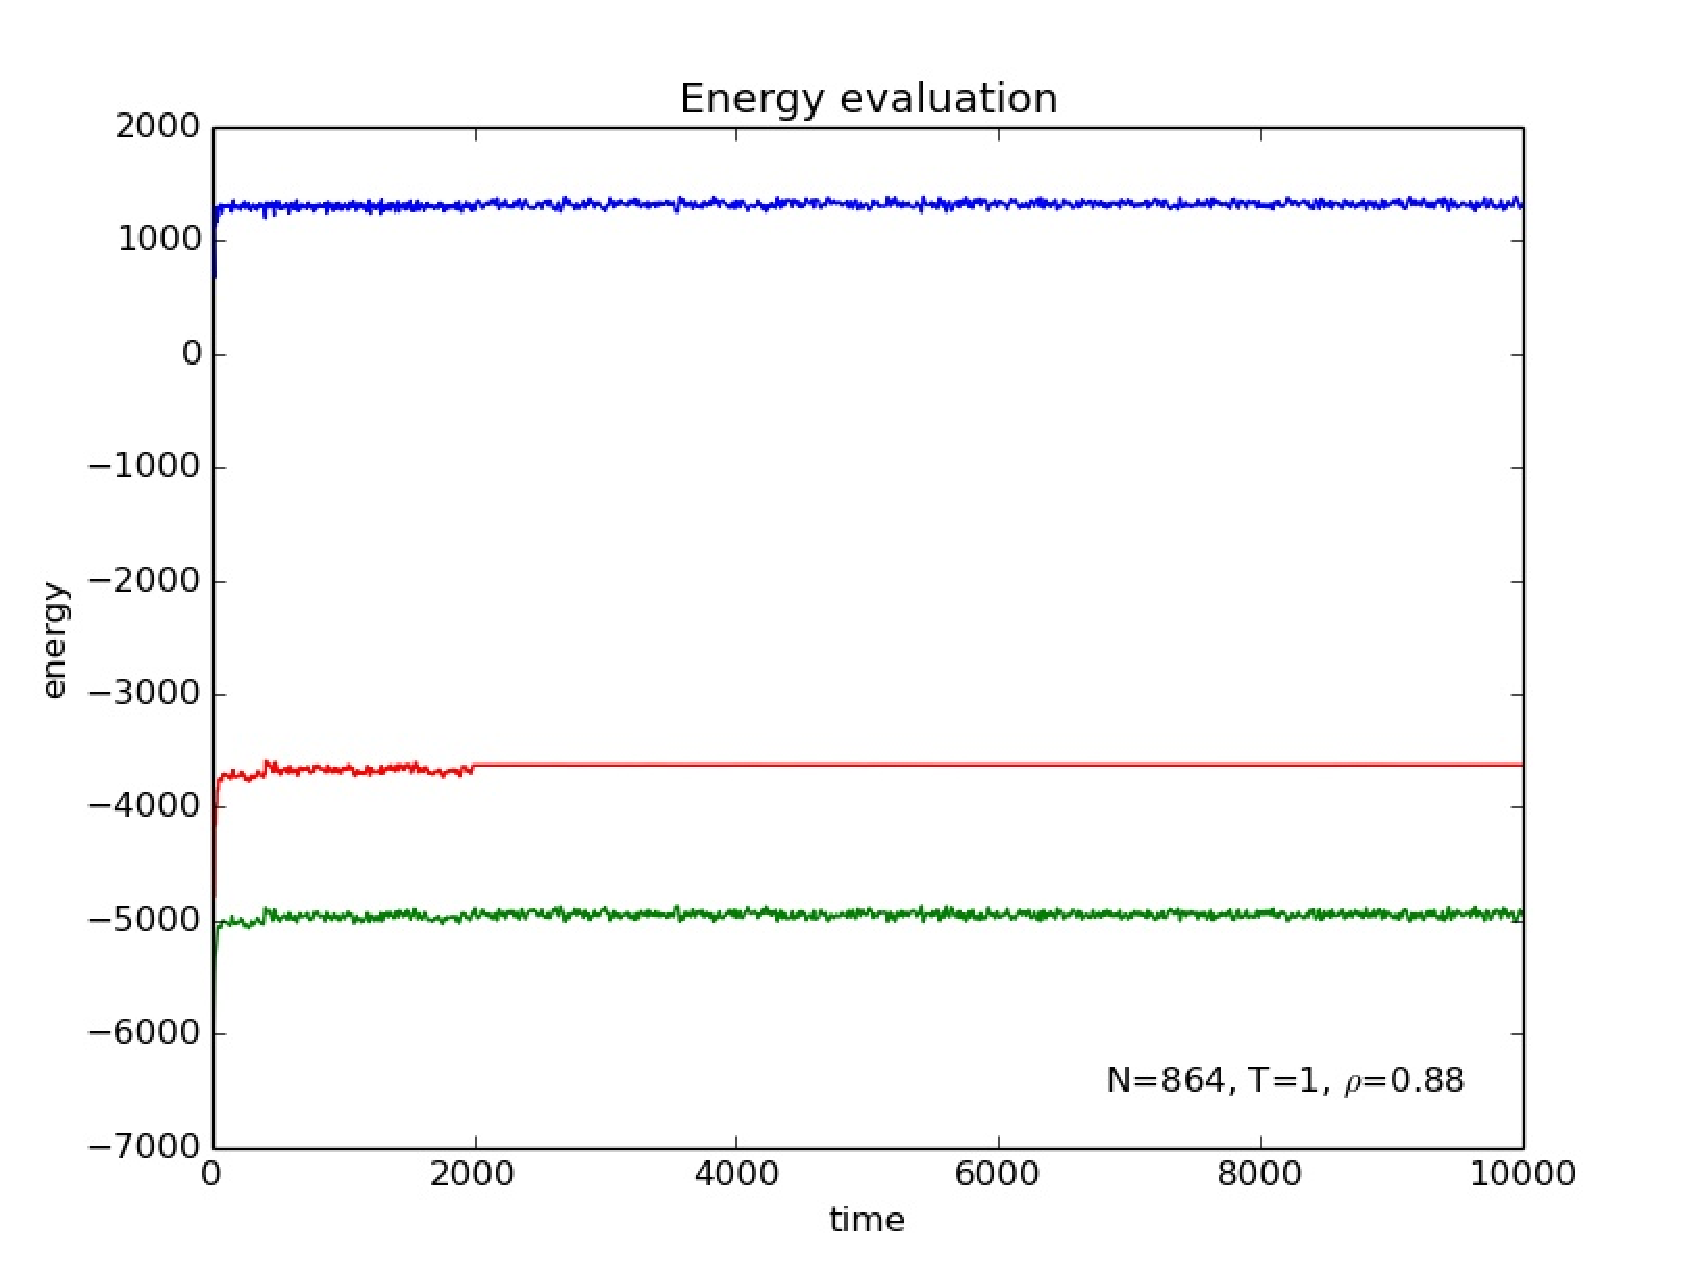
\includegraphics[width=\linewidth]{plots/energyT1rho088N864lpnum1000.pdf}
\caption{Energy as a function of time step for 864 particles, with $T=1$ and $\rho = 0.88$.  The blue line is the total energy, the red line is the \textbf{WHAT} and the green line is \textbf{WHAT}.}
\label{engcons}
\end{center}
\end{figure}

Temperature is another variable that must be kept in a reasonable range.  Because, we have taken $k_B =1$, energy and temperature are measured with the same units.  If we take this to be electron volts, the conversion factor is $1 $ eV $\approx 11600$ K.  Thus, as temperature increases, we quickly enter a realm where the particles are traveling at relativistic speeds.  Our simulation is purely classical and thus not equipped to accurately calculate relativistic simulations.

\subsection{Thermostat}

Using the renormalization method explained in Section \ref{thermo}, we were able to bring our system to any given target temperature (non-relativistic) from any starting temperature.  Some of these target temperatures that are used in the following calculations are given in Table 1.  \\

\begin{table*}
\begin{center}
\begin{tabular}{| c | c | c | c |}
\hline $T_{targ}$ [eV] & $T$ [eV] & $\sigma_T$ [eV] & $SE_T$ [eV] \\ \hline
 0.5 & 0.499830 & 0.009934 & 0.000111 \\ \hline
1.0 & 1.015010 & 0.018228 & 0.000203  \\ \hline
3.0 & 2.975473 & 0.032667 & 0.000365 \\ \hline
\end{tabular}
\label{temptable}
\caption{Calculated temperatures, $T$, for each target temperature, $T_{targ}$, and their uncertainties $\sigma$, given as $T \pm \sigma$, used throughout the remainder of the calculations.  $SE_T$ gives the difference between the calculated temperature ($T$) and the target temperature.}
\end{center}
\end{table*}

Based on how often the velocity was renormalized, the temperature could be brought more slowly or quickly to the target temperature.  \textbf{include plots - every step, every 10 steps, every 100 steps, and maybe a little more discussion on this point.}

\begin{figure}[H]
\begin{center}
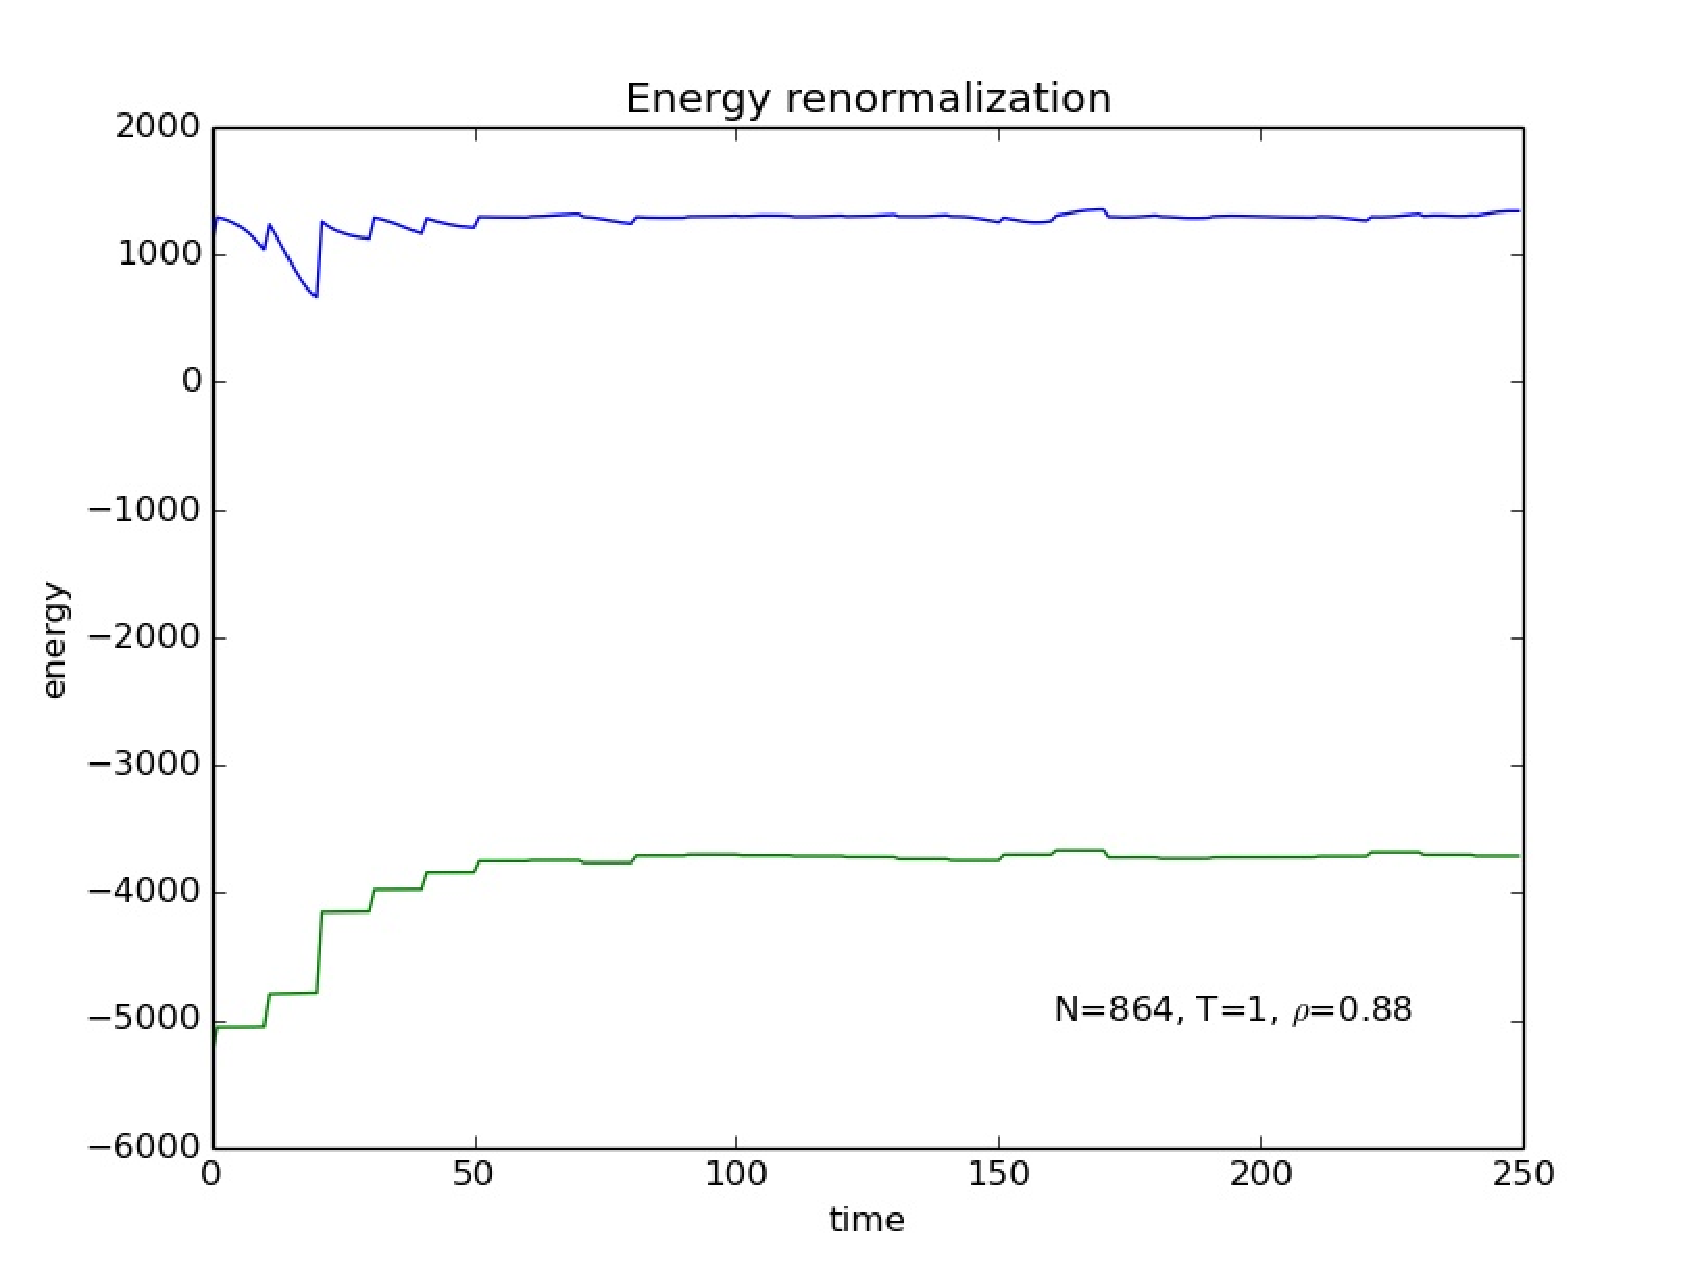
\includegraphics[width=\linewidth]{plots/renormalizationshorttimerange.pdf}
\caption{Plot of the renormalized energy (calculated with the renormalized velocity) over 250 time steps.  The green line is \textbf{What?} and the blue line is \textbf{What?}}
\label{engrenorm}
\end{center}
\end{figure}

\subsection{Correlation Function}

Once a thermostat was established, correlation functions could be calculated.  As mentioned earlier, these give us a sense of what state of matter our system is in for different combinations of temperatures and densities.  At a low temperature and relatively high density, we confirmed that our system had properties of a solid (Figure \ref{corsolid}), at intermediate temperatures and densities, our system had properties of a liquid (Figure \ref{corliquid}), and at a high temperature and low density, our system displayed properties of a gas (Figure \ref{corgas}).  

\begin{figure}[H]
\begin{center}
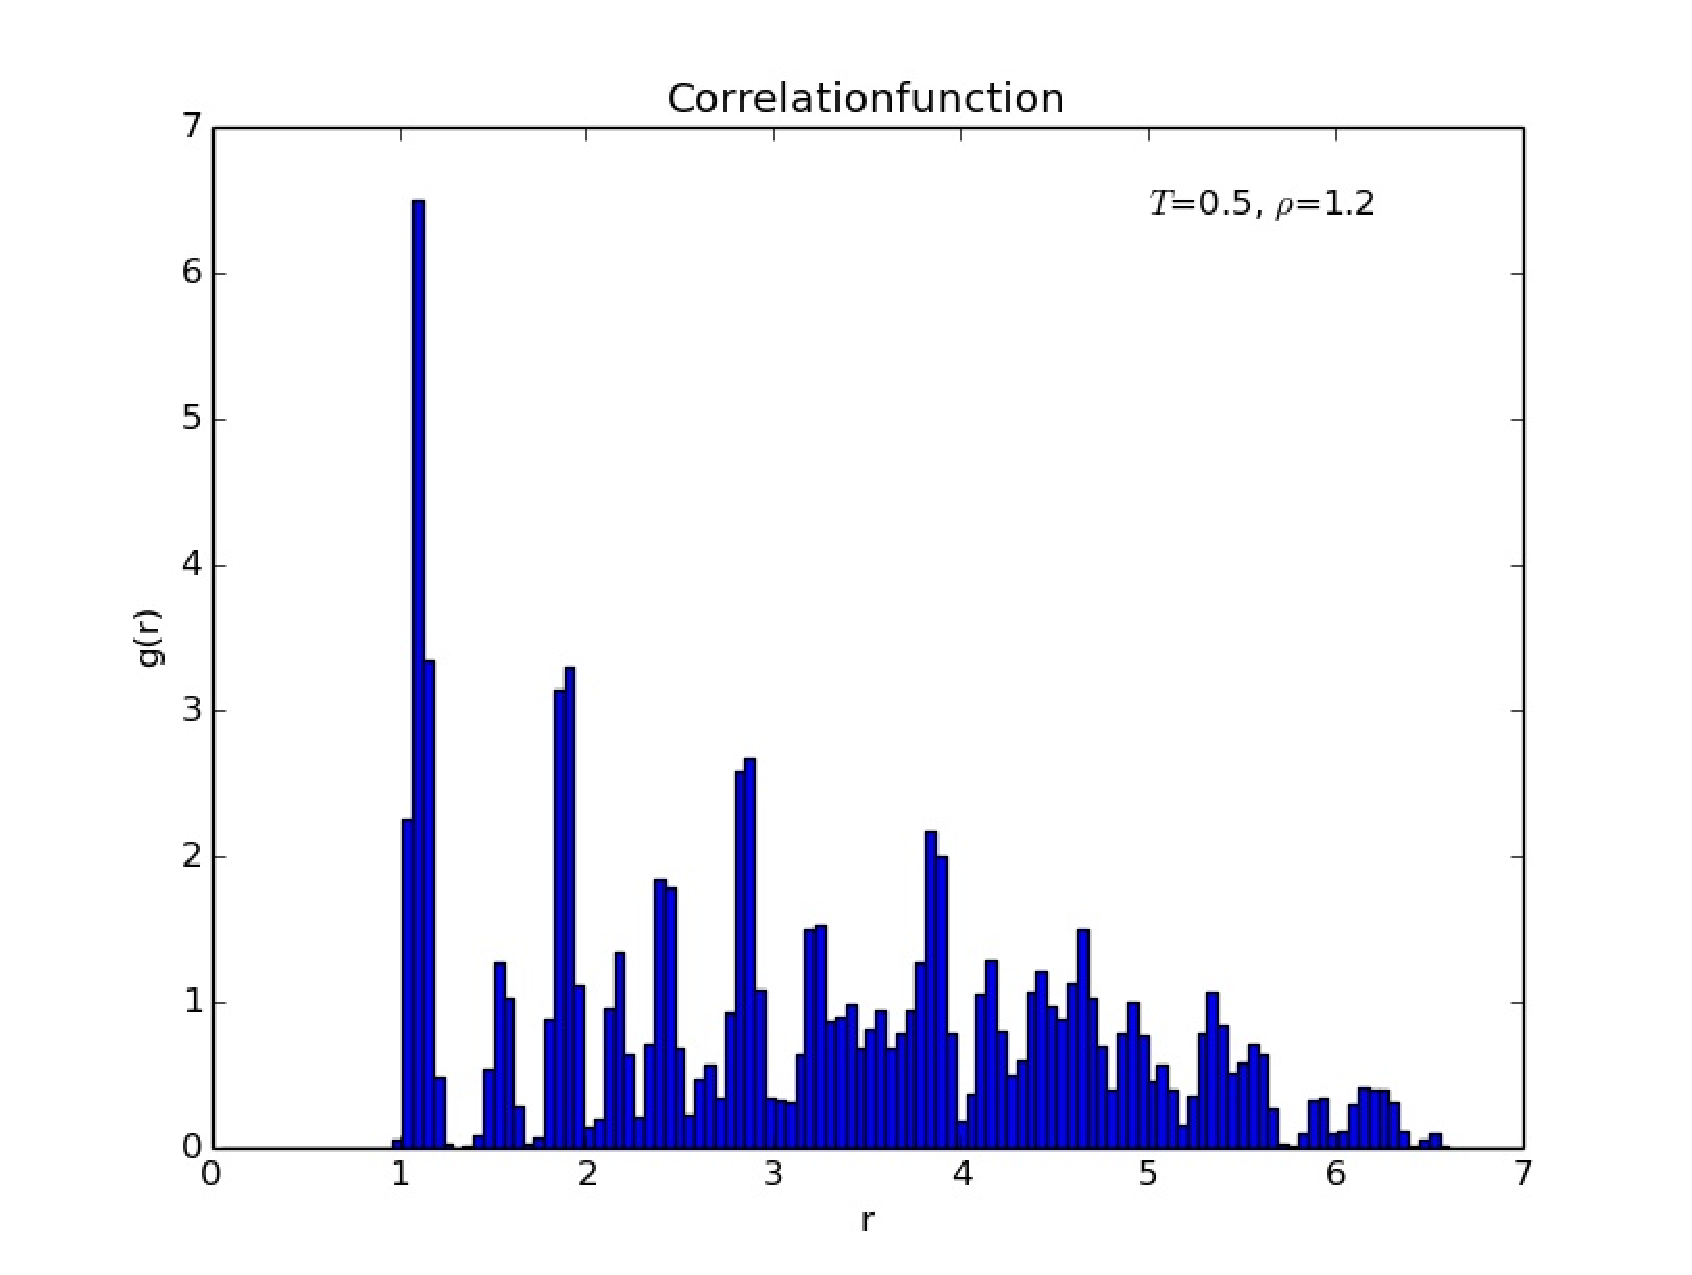
\includegraphics[width=\linewidth]{plots/correlationfunctionT05rho12x.pdf}
\caption{Correlation function for a solid at $T=0.5$ and $\rho=1.2$.  This periodic structure is what we would expect from a solid.}
\label{corsolid}
\end{center}
\end{figure}

\begin{figure}[H]
\begin{center}
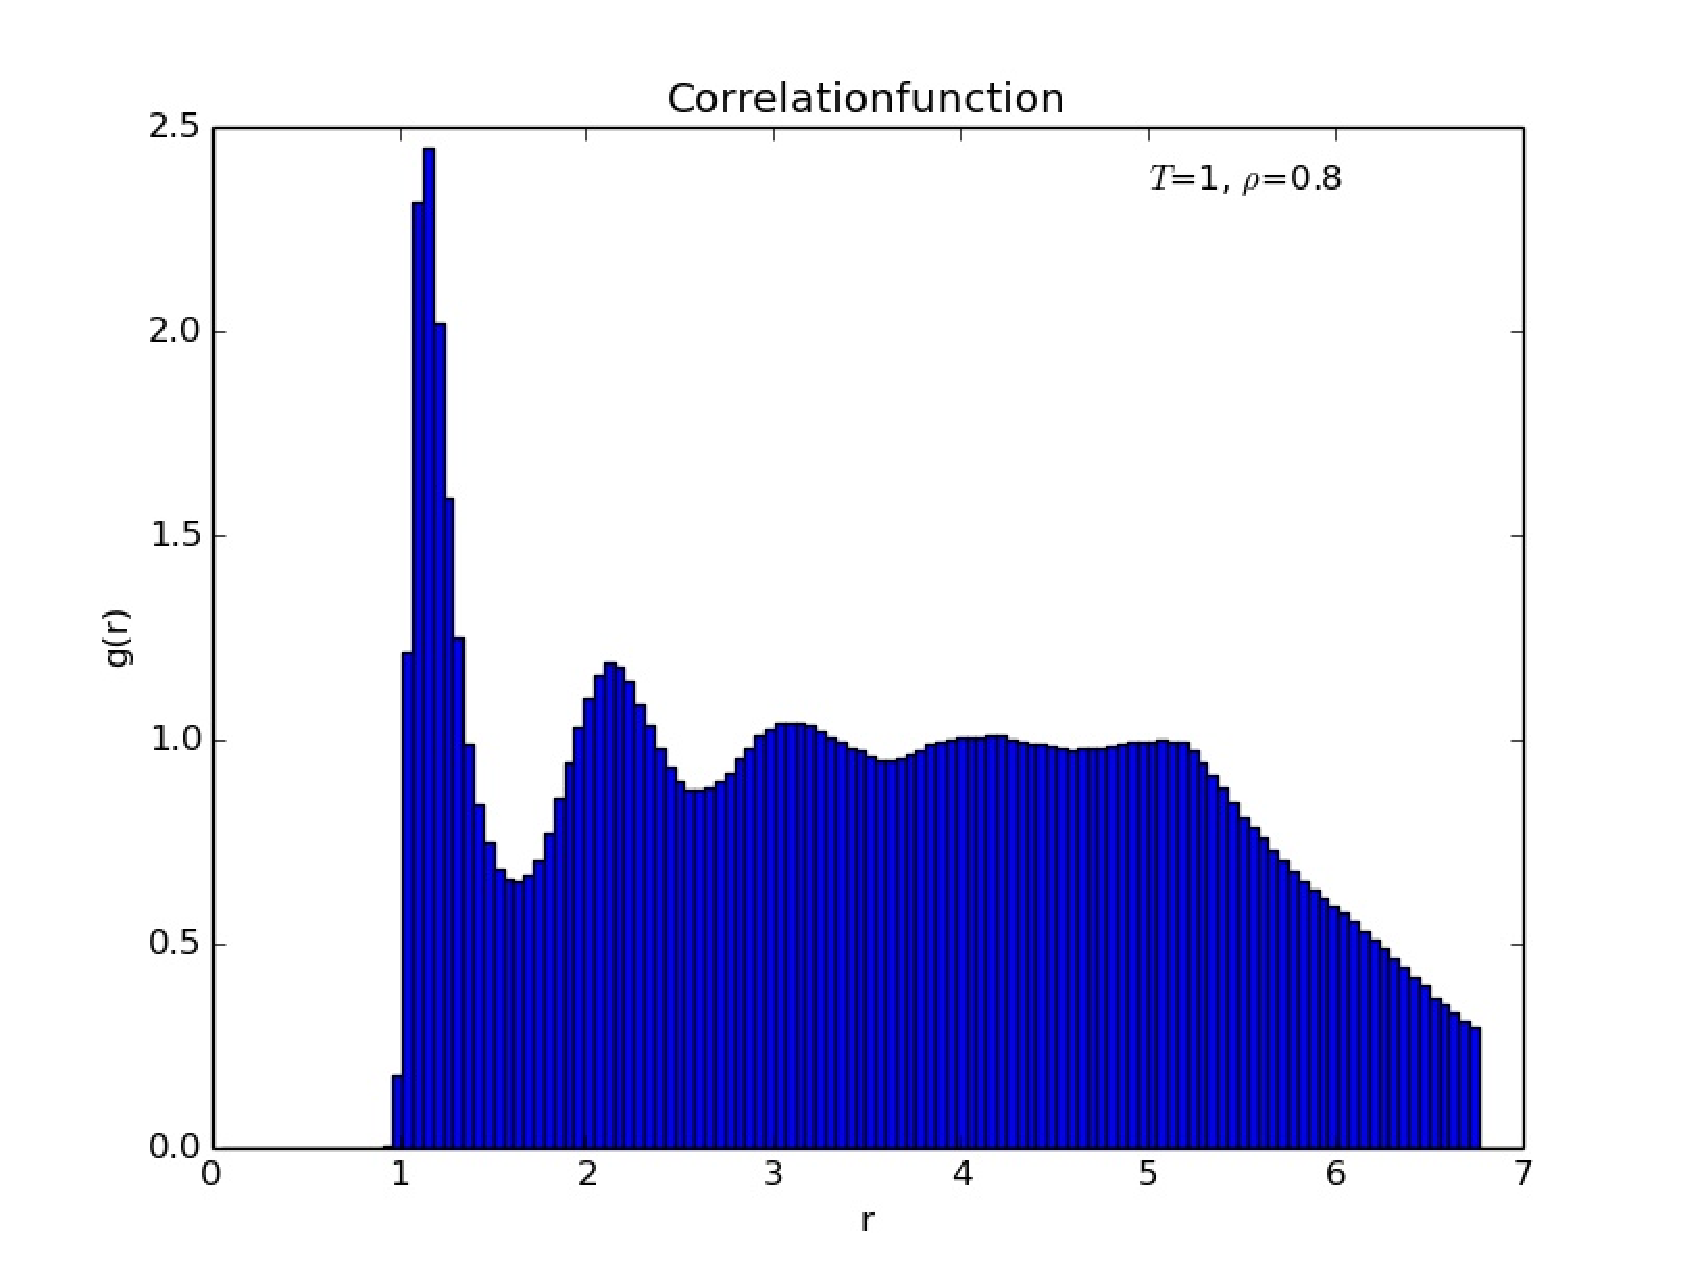
\includegraphics[width=\linewidth]{plots/corfunct1rho08n864lp500.pdf}
\caption{Correlation function for a liquid at $T=1$ and $\rho=0.5$.  We can see from Figures \ref{corsolid} and \ref{corgas} that this phase is in between the other two, as a liquid is considered to be in between a solid and a gas.}
\label{corliquid}
\end{center}
\end{figure}

\begin{figure}[H]
\begin{center}
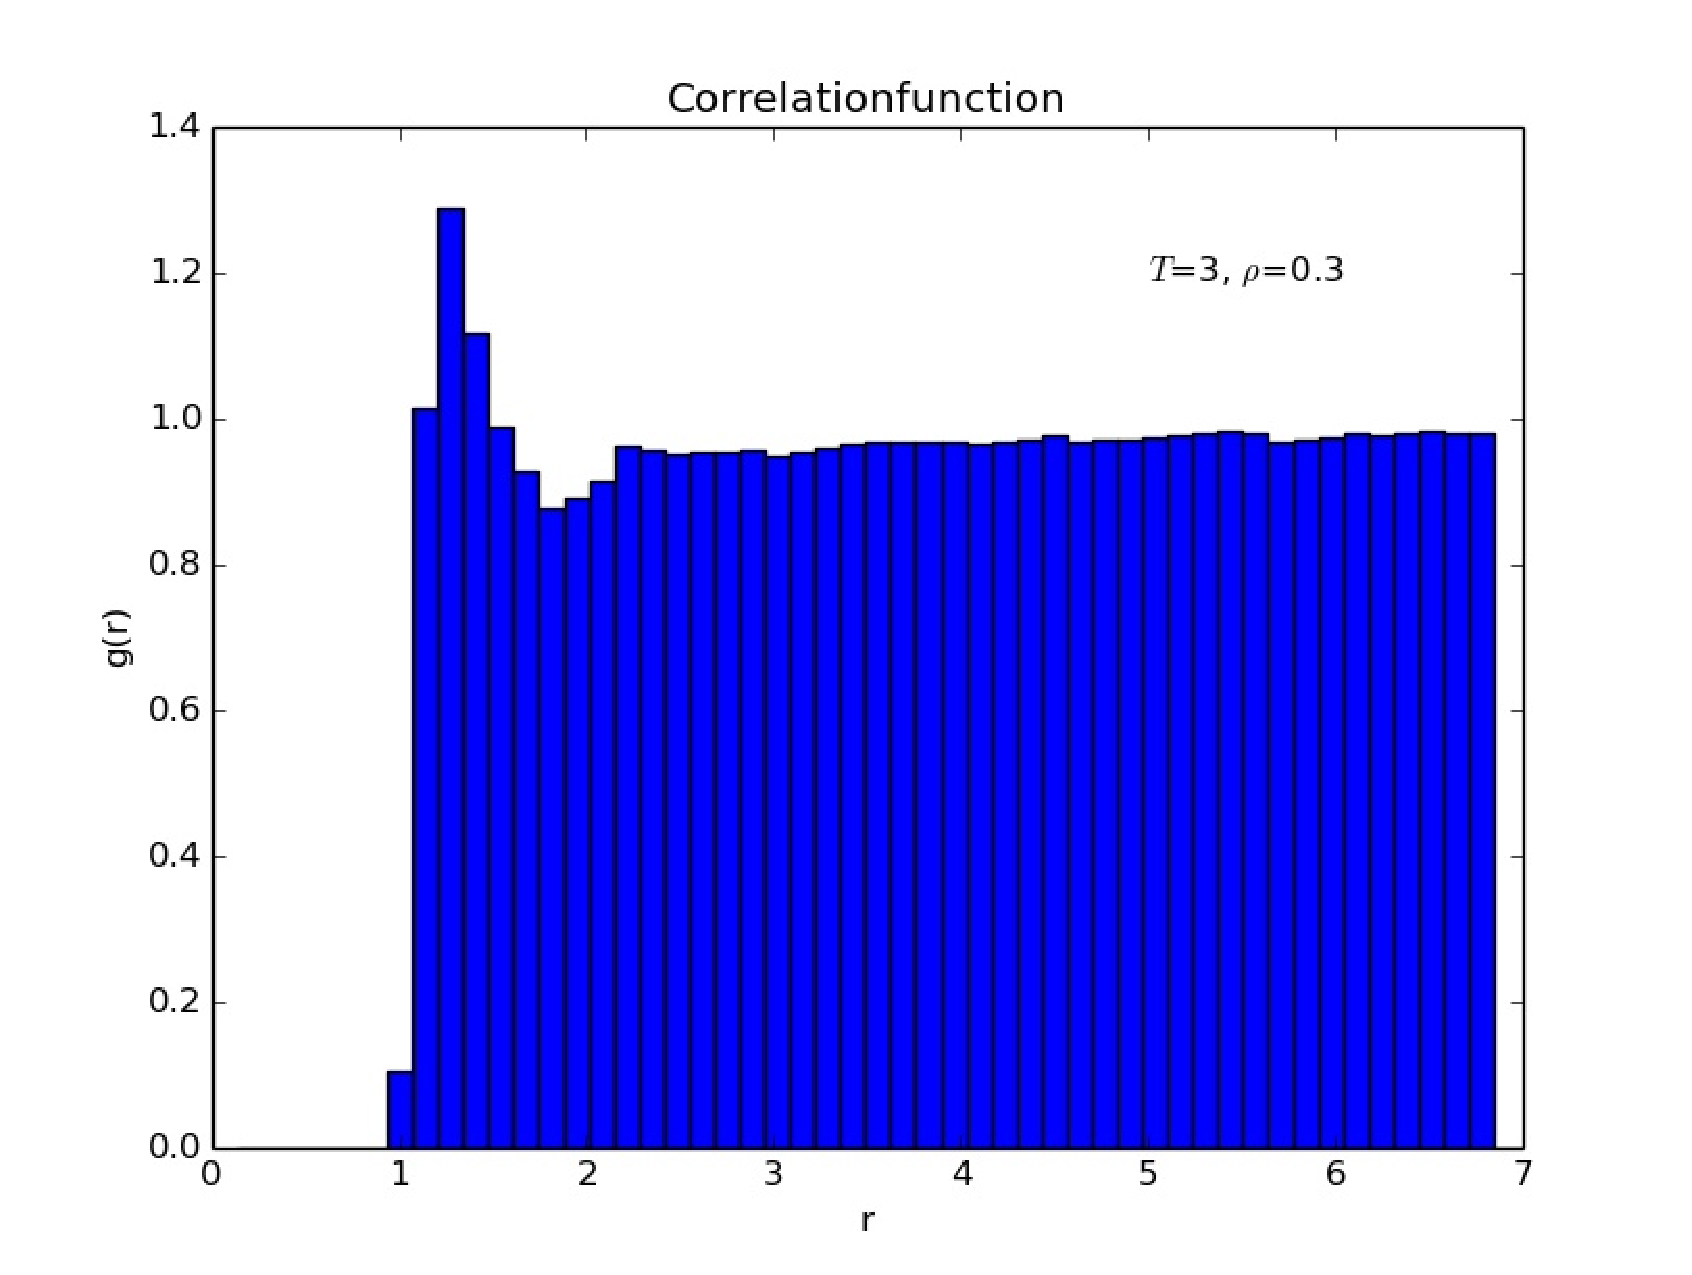
\includegraphics[width=\linewidth]{plots/correlationfunctionT3Rho03x.pdf}
\caption{Correlation function for a gas at $T=3$ and $\rho = 0.3$.  The exponential decay is the shape that we would expect.}
\label{corgas}
\end{center}
\end{figure}

\textbf{One for each of the three states of matter - can either keep the same density and run the calculation for different temperatures or take one temperature and see if we can find different densities at which each state of matter exists.  Both are probably interesting.}

\subsection{Pressure}

\begin{table*}
\begin{center}
\begin{tabular}{| l | c | c | c | c | r |}
\hline  $T$ & $\rho$ & $P$ & $\sigma_{pressure}$ & $\sigma_{pressureblock}$ & $\sigma_{pressureblock}/ \sqrt n$ \\ \hline
  3 & 0.5 & 5.4862 & 0.0836 & 0.0089 & 0.0010 \\ \hline
  1 & 0.88 & 2.6982 & 0.0171 & 0.0067 & 0.0008 \\ \hline
  0.5 & 1.2 & 1.1105 & 0.0056 & 0.0021 & 0.0002 \\ \hline
\end{tabular}
\label{pressuretab}
\caption{Pressure of a gas, solid, and liquid (top to bottom), at a given temperature $T$ and density $\rho$.  $\sigma$ gives the standard deviation of each calculation.  \textbf{Explain the difference between each of the sigma values.}  Numbers can be compared to \cite{thijssen}.}
\end{center}
\end{table*}

\textbf{sorry for the ugly indent, but these are the numbers we can work with. We should add that are results lie close to those obtained by the method Jos has used. He finds for T = 1, rho = 0.88 a value of 2.98 for p/rho. If we divide our p by rho, we get: 3.07. Sadly enough it is not exactly the same, but ok. sorry i couldn't write this nicely, i'm a bit to tired.}\\

\textbf{This (above) should go into the report when talking about the pressure calculations.}

\section{Conclusion}
\label{conc}

In conclusion, we successfully ran a molecular dynamics simulation of 108 argon atoms.  Beginning in an fcc crystalline lattice with periodic boundary conditions, we simulated contact with thermostats of $T=0.49983 \pm 0.009934$ eV, $T= 1.01501 \pm 0.018228$ eV, and $T=2.975473 \pm 0.03267$ eV.  From there, we calculated calculated properties of a gas at $T=3$ eV, $\rho=0.3$ $\AA ^{-3}$ with $P=5.4862 \pm $ eV$\AA^{-3}$, a liquid at $T=1$ eV, $\rho =0.8$ $\AA ^{-3}$ with $P=2.6982 \pm $ eV$\AA^{-3}$, and a solid with $T=0.5$ eV, $\rho=1.2$ $\AA ^{-3}$ at $P=1.1105 \pm $ eV$\AA^{-3}$.  With the exception of some of the pressure values, our current calculations agree with those of \cite{thijssen} under similar conditions.  \\

Further work can still be done.  There are other interesting thermodynamical quantities that can be calculated for this system, such as the specific heat, chemical potential, and free energy.  It would also be interesting to change the initial conditions of the system.  Instead of periodic boundary conditions, put the system in a physical box and see how the interactions with the wall change the observables.  Also, a different crystalline structure (such as hcp) could be used as the initial configuration.  This would allow us to see whether the system did rearrange itself into the true fcc ground state of argon.  Even with all of these possibilities, we provided a realistic molecular dynamics simulation of argon.  

\appendix 

\section{Error Calculations}

Like experimental measurements, numerical calculations should include error bars.  Just as in an experiment where we would ideally take many measurements and calculate an error based on their standard deviations from the mean, we can use the same concept to put error bars on our calculated values.  There are many ways that these uncertainties can be calculated, but in this paper, we will be using a result of the ergodic theorem \cite{Birkhoff}, that the spatial average is equal to the time average.  \\

There are several ways that we can calculate a time average for our calculation.  Perhaps, the most obvious one is to run the calculation several times to generate a mean and a standard deviation.  However, this process is lengthy and can be heavily dependent on the seed of the random number generator used in initializing positions and velocities the particles.  \\

\begin{figure}[H]
\begin{center}
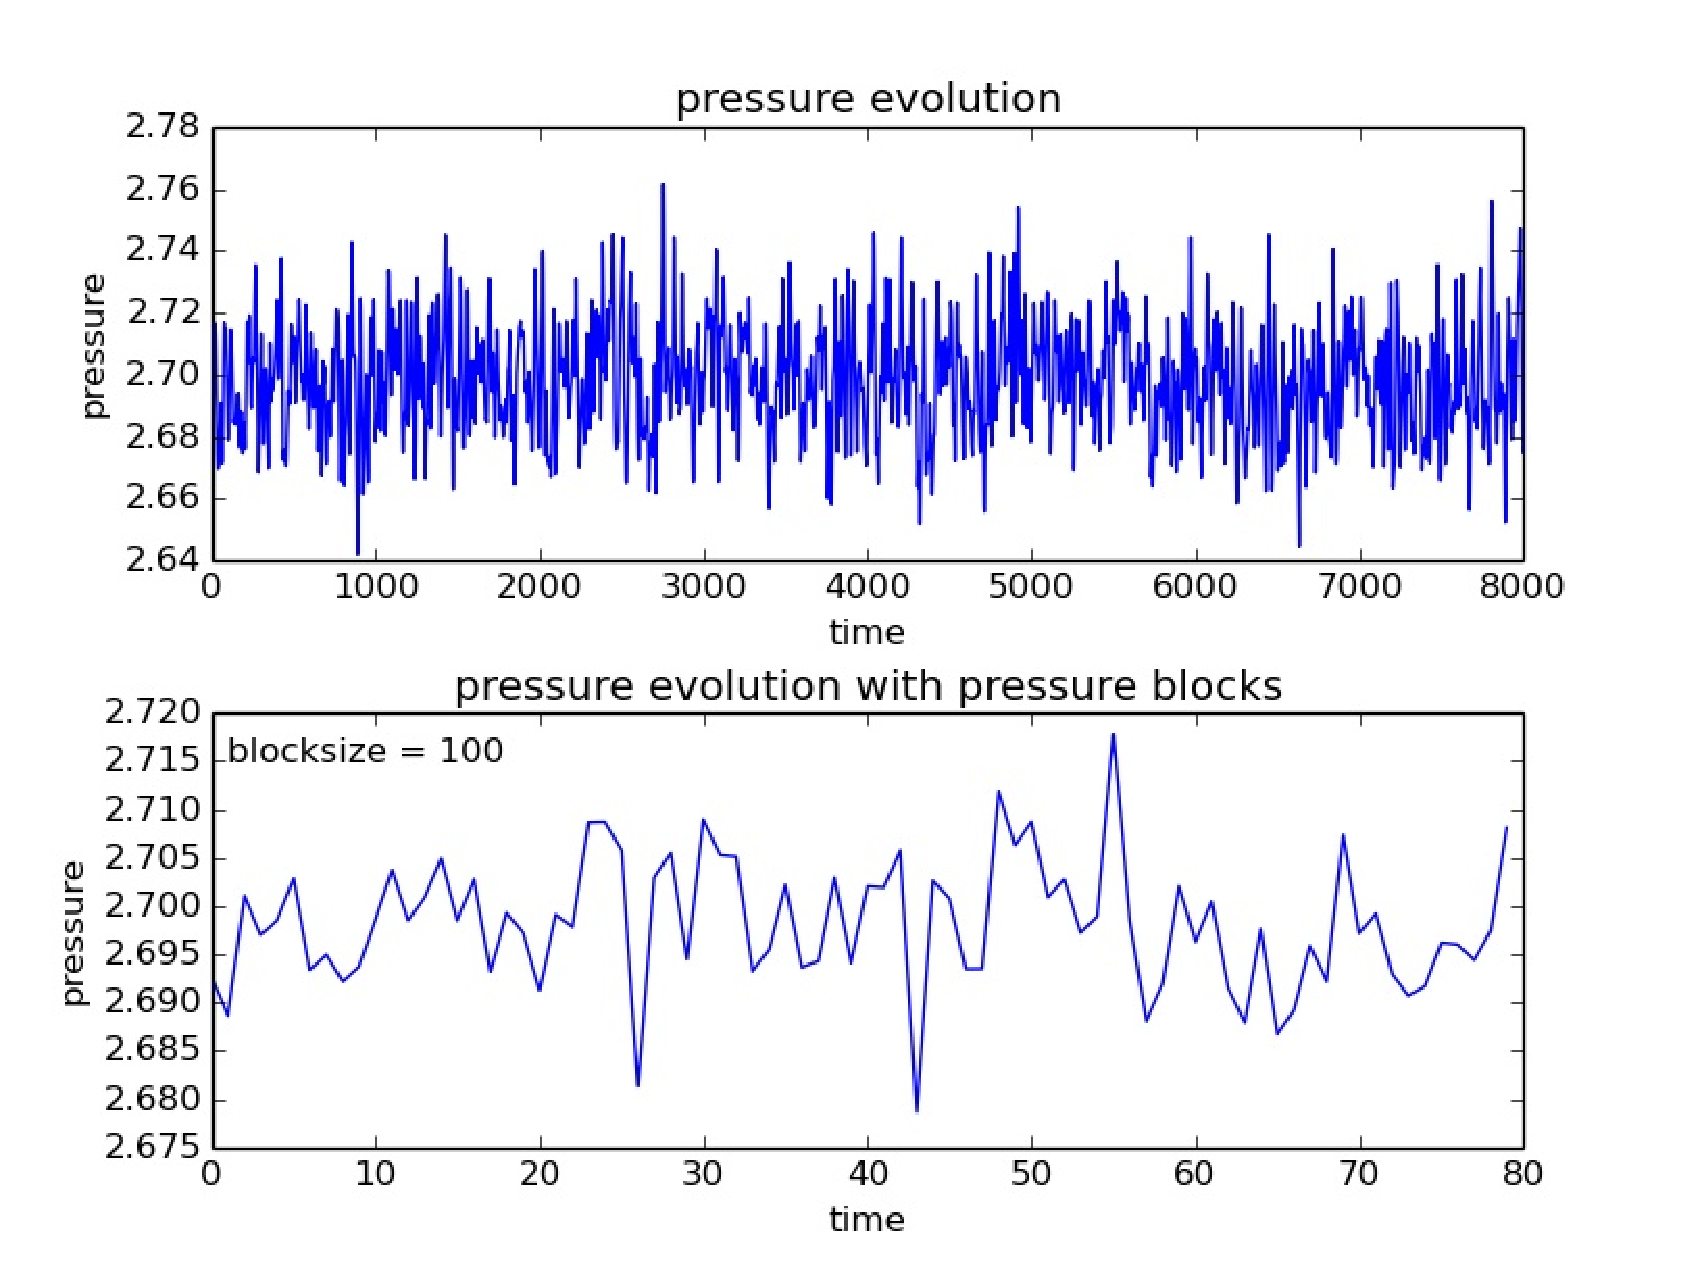
\includegraphics[width=\linewidth]{plots/presn100lp10000T1rho088prt864.pdf}
\caption{Top, pressure calculated for every time step.  Bottom, pressure averaged over every 100 time steps in the top plot.  }
\label{errex}
\end{center}
\end{figure}

It is, therefore, much better to run one simulation and average over many blocks of time.  In each simulation, after a long enough period of time, the quantity of interests will settle on some mean value with every time step oscillating around this value, as show in Figure \ref{errex}.  While each value depends on the previous value, averaging over a large enough number of time steps will produce a value independent of the previous block of time steps.  For each of these blocks, 100 time steps, an average is calculated (this is equivalent to having many measurements from an experiment), and then from each of these "measurements", we can calculate an average value for our simulation and an error for that value.  The average value is defined as 

\begin{equation}
\bar{C} = \frac{1}{N}\sum \limits _{i=1}^N C_i 
\end{equation}

\noindent and the error is calculated from 

\begin{equation}
\sigma ^2 = \frac{1}{N}\sum \limits _{i=1}^N (C_i - \bar{C})^2
\end{equation}

\noindent where $\sigma$ is the error on a given quantity, $N$ is the number of time-step blocks, and $C_i$ is the quantity value for each time step block.\\

This ensures that we include fluctuations in the numbers that we report, as well as account for a decreasing error with an increasing number of "measurements".  

\end{multicols}

\bibliography{MolDynBib}

%\begin{thebibliography}{99}

%\bibitem{deGroot}
  %B. de Groot,
  %Computational Biomolecular Dynamics Group, Max Planck lnstitute for Biophysical Chemistry. %Retrieved from http://www3.mpibpc.mpg.de/groups/de_groot/
  
%\bibitem{thijssen}
 % Thijssen, J.M.(2007). Computational Physics. Cambridge, Cambridge University Press.
%\end{thebibliography}

\end{document}
